\columnbreak
\section*{\begin{tabular*}{\linewidth}{@{}l @{\extracolsep{\fill}} r@{}}
		Nr.~17 & MUN~87/2-1-3 \\
	\end{tabular*} 
}

\textsf{\textbf{Munda (Likwala-aux-Herbes; Fpl.~304)}}

\vspace{1em}

\noindent\begin{tabular}{@{}rl@{}}
	\textbf{Feldarbeit:} & \textbf{24.08.--30.08.1987 (H. Holsten)} \\ 
	\textbf{Abb.:} & \textbf{\ref{fig:MUN87.2-1-3_Plana_Fotos}--\ref{fig:MUN87-2-1-3_14C_OxCal}} \\ 
	\textbf{Tab.:} & \textbf{\ref{tab:MUN87-2-1-3_Funde}--\ref{tab:MUN87-213_14C-Daten}}\\
	\textbf{Taf.:} & \textbf{92.1--93.8} \\ 
	\textbf{Lit.:} & \textbf{--} \\ 
\end{tabular} 

\paragraph{Grabung und Befunde}\hspace{-.5em}|\hspace{.5em}%
Etwa 0,35\,m nördlich des Befundes MUN~87/2-1-1 (Kat.-Nr.~16) wurde an der Oberfläche eine weitere Verfärbung sowie Gefäßfragmente beobachtet. In Verlängerung der für die Ausgrabung von MUN~87/2-1-1 angelegten Profilachse wurde auch dieser zweite, als MUN~87/2-1-3 bezeichnete Befund ausgegraben (Abb.~\ref{fig:MUN87.2-1-3_Planum+Profil_Zeichnung}). Durch die Grabung wurde eine zirka 1,4\,m tiefe Grube erfasst, die einen Durchmesser von etwa 0,8~m hatte.\footnote{Die östliche Hälfte wurde bis etwa 0,8\,m unter der Oberfläche in künstlichen Abträgen ausgegraben. Ab dieser Tiefe lief der Befund in das Profil und konnte nicht mehr erfasst werden. Nach der zeichnerischen Dokumentation des Profils wurde die westliche Hälfte den Schichten aus dem Profil folgend ausgegraben. Wo im Profil keine ausreichende Differenzierung von Schichten möglich war,< wurden künstliche Abträge angelegt. Die Position der gefundenen Gefäße wurde auf Fotos sowie in Handskizzen festgehalten. Aufgrund starker und tagelanger Regenfälle war die systematische Ausgrabung und Dokumentation der westlichen Befundhälfte nur deutlich eingeschränkt möglich.} Sie enthielt eine intentionelle Deponierung aus 15 auf der Mündung oder Seite liegenden Gefäßen des Pikunda-Munda-Stils \parencite[siehe][]{Wotzka.1993}.\footnote{Zu intentionellen Deponierungen in Gruben im östlich an das Arbeitsgebiet angrenzenden Innern Kongobecken siehe \textcite{Wotzka.1993}.}

\begin{figure*}[p]
	\centering
	\begin{subfigure}[t]{\columnwidth}
		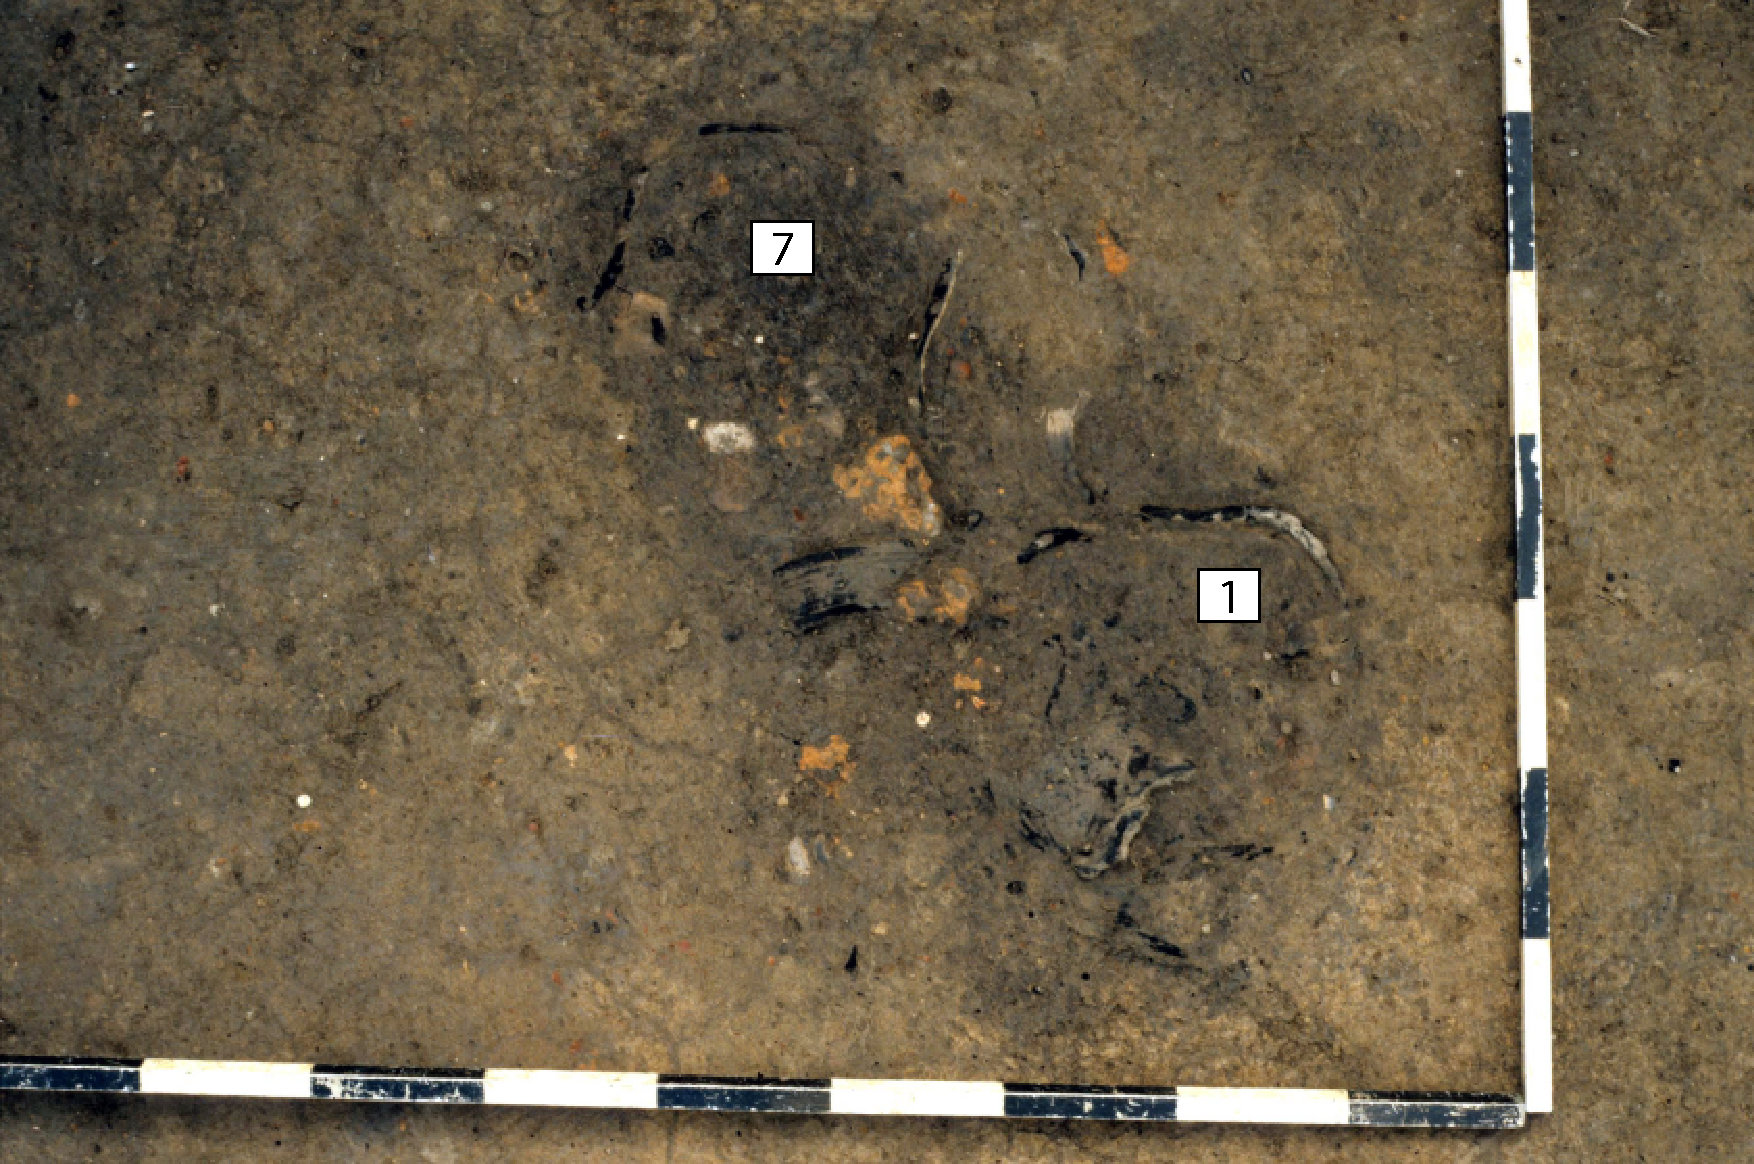
\includegraphics[width = \textwidth]{fig/MUN87-213_T41_F87-02-14.pdf}
		\caption{T41 (Oberfläche; Foto: F. Nikulka, 1987).}
		\label{fig:MUN87-213_T41_F87-02-14}
	\end{subfigure}\hfill
	\begin{subfigure}[t]{\columnwidth}
		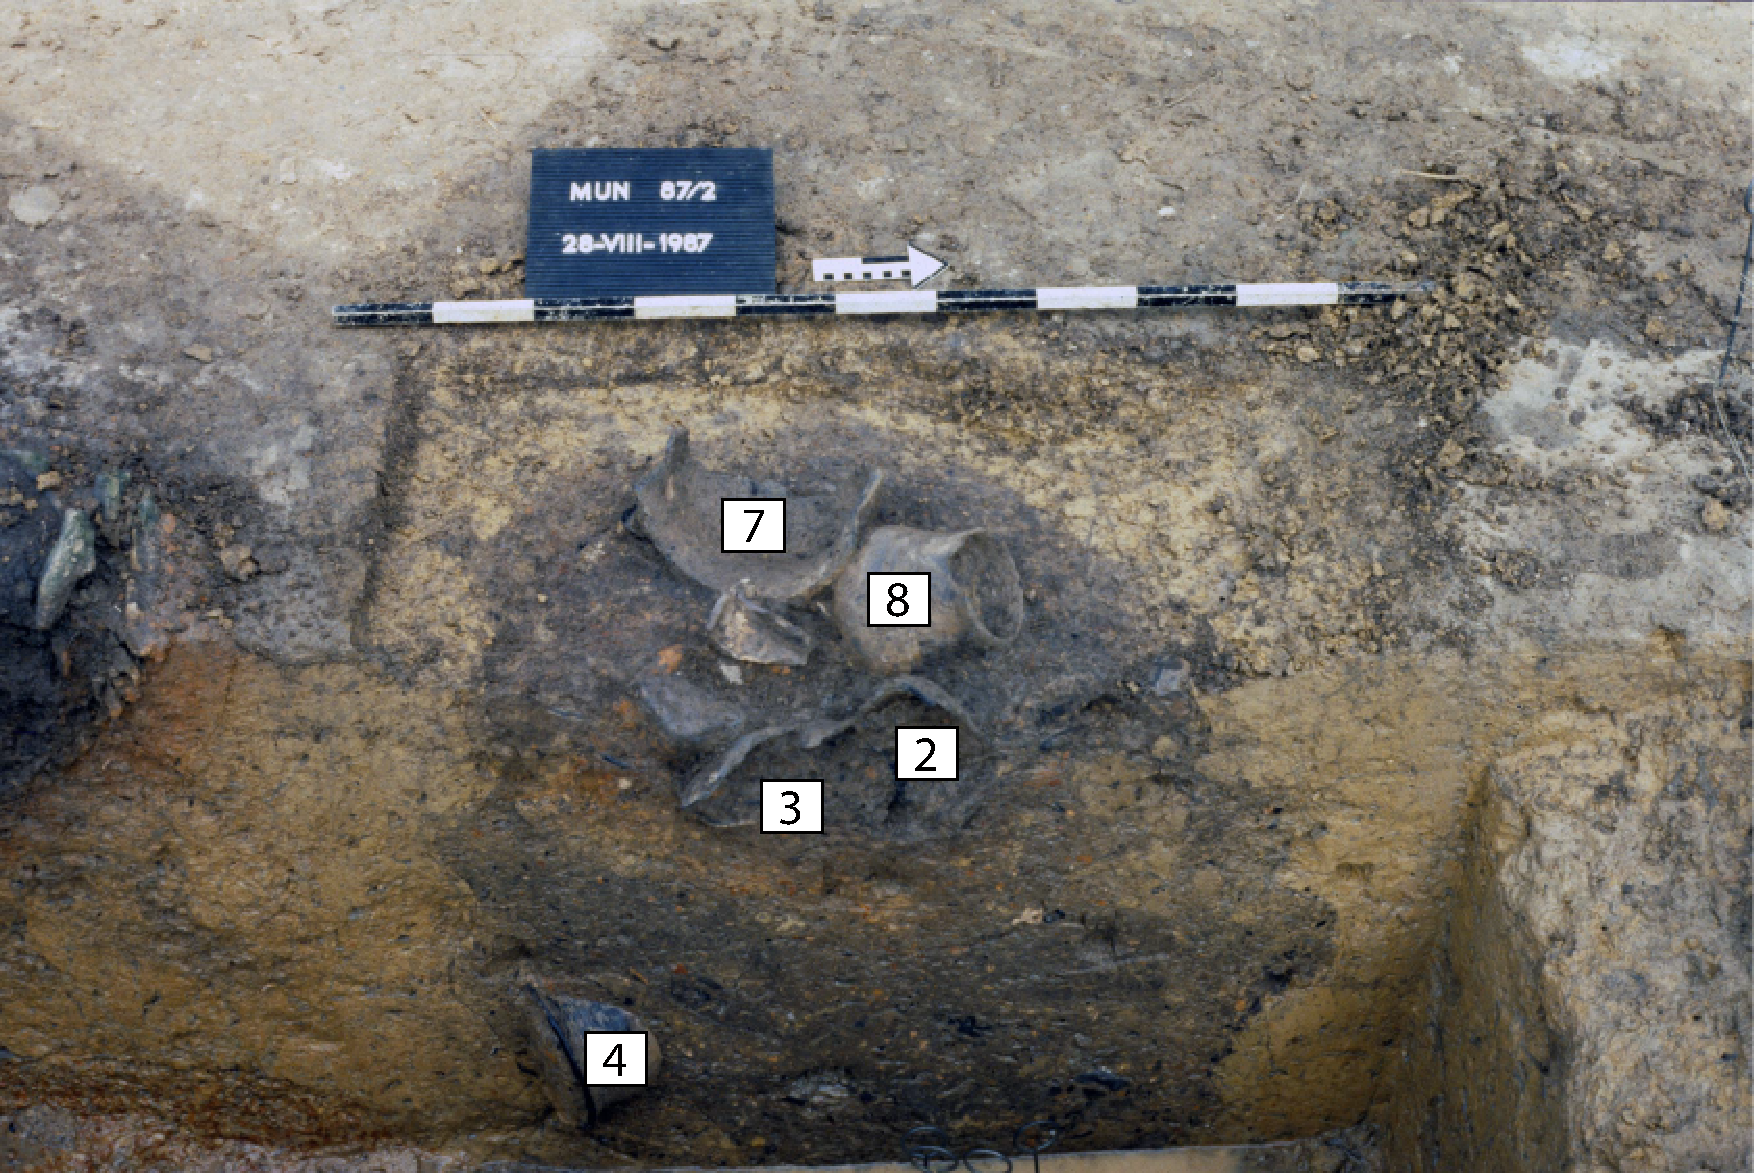
\includegraphics[width = \textwidth]{fig/MUN87-213_T49_T49_H87-06-8.pdf}
		\caption{T49 (Foto: H. Holsten, 1987)}
		\label{fig:MUN87-213_T49_T49_H87-06-8}
	\end{subfigure}
	\begin{subfigure}[t]{\columnwidth}
		\includegraphics[width = \textwidth]{fig/MUN87-213_T53_H87-05-29.pdf}
		\caption{T53 (Foto: H. Holsten, 1987)}
		\label{fig:MUN87-213_T53_H87-05-29}
	\end{subfigure}\hfill
	\begin{subfigure}[t]{\columnwidth}
		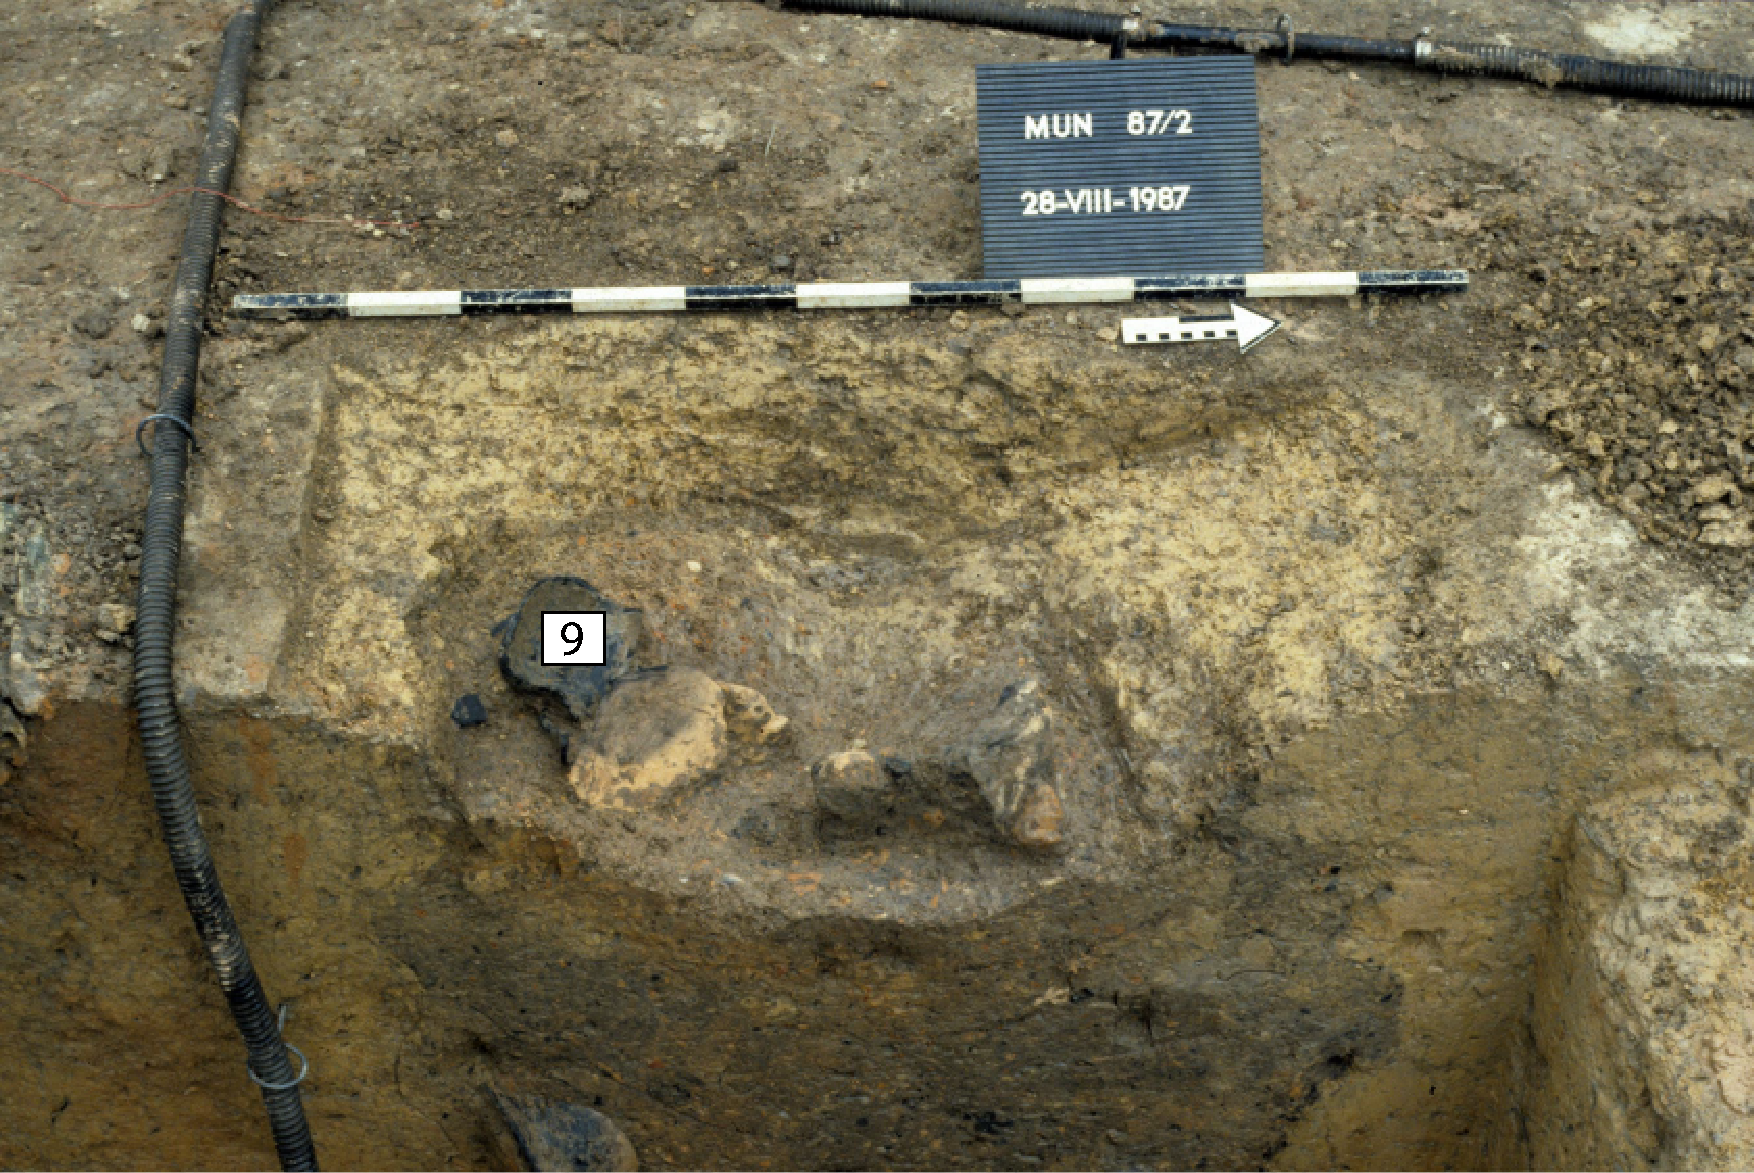
\includegraphics[width = \textwidth]{fig/MUN87-213_T64_H87-06-11.pdf}
		\caption{T64 (Foto: H. Holsten, 1987)}
		\label{fig:MUN87-213_T64_H87-06-11}
	\end{subfigure}
	\begin{subfigure}[t]{\columnwidth}
		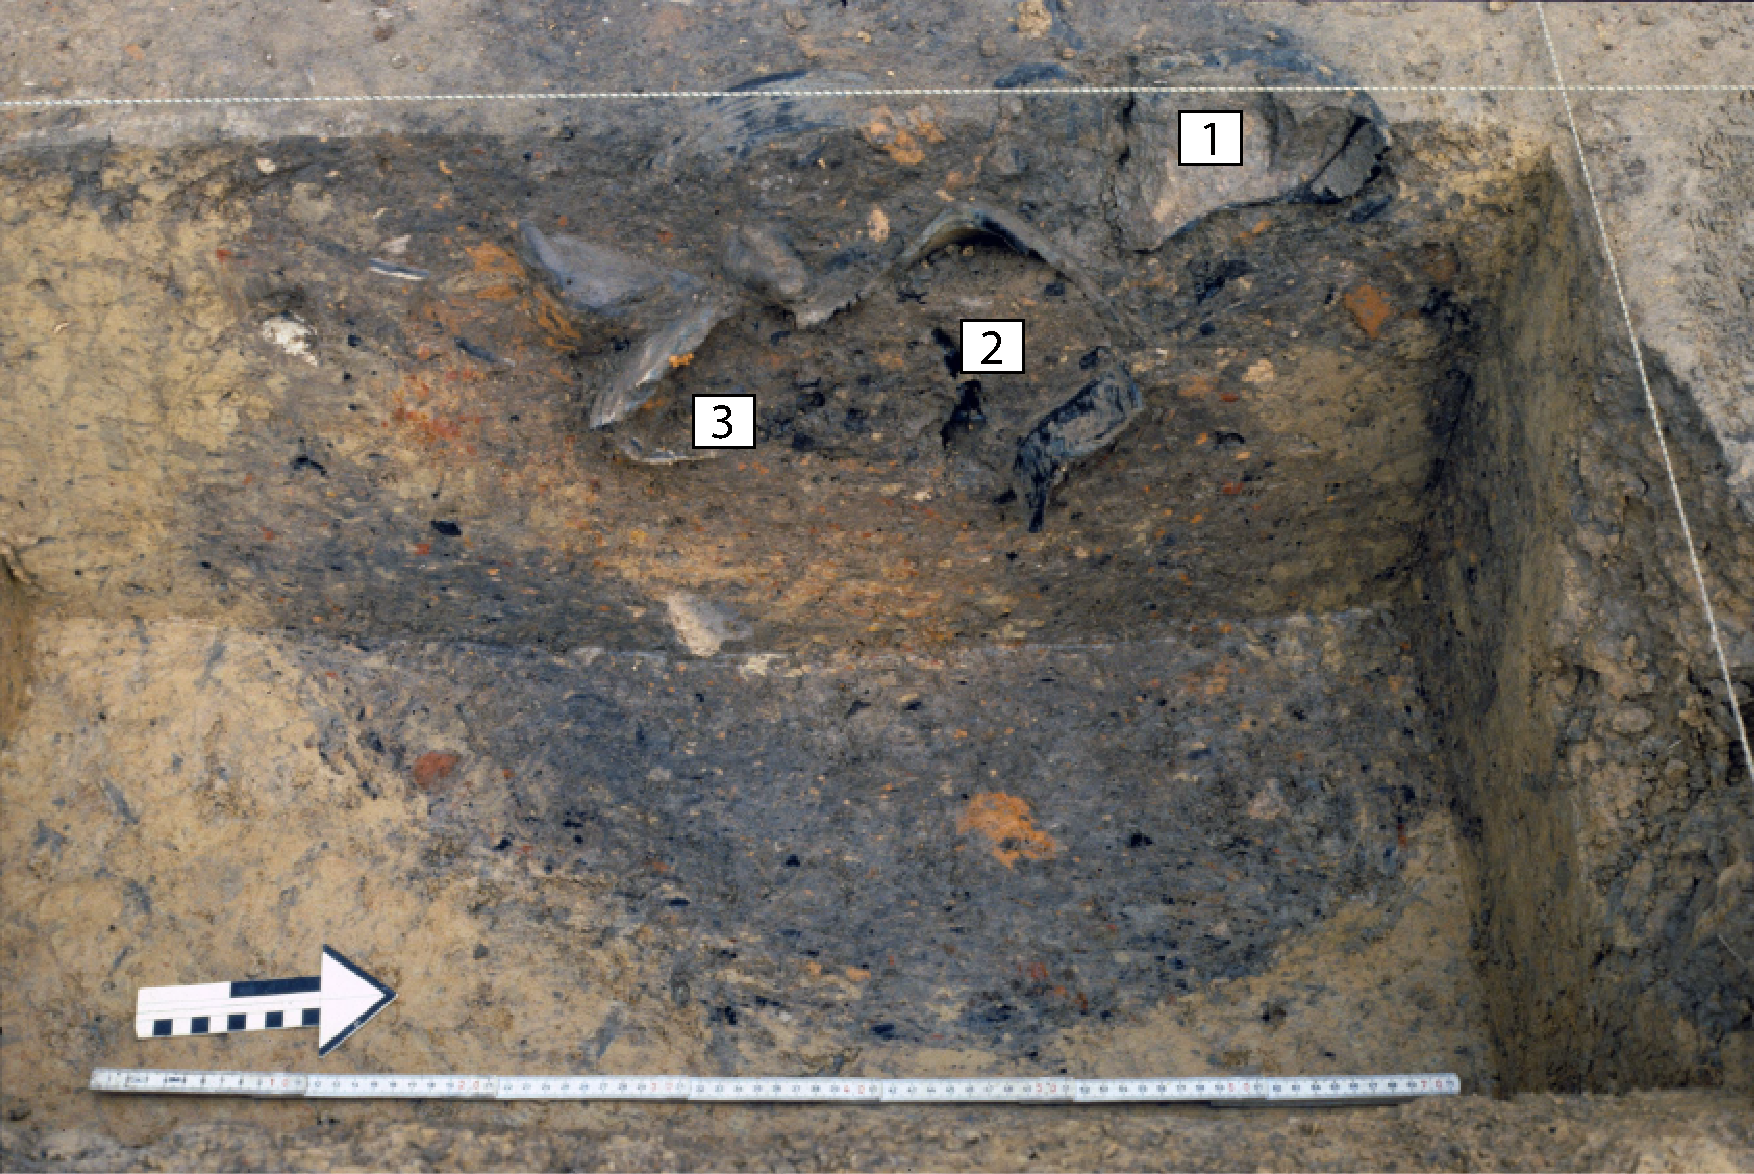
\includegraphics[width = \textwidth]{fig/MUN87-213_T72_H87-06-3.pdf}
		\caption{T72 (Foto: H. Holsten, 1987)}
		\label{fig:MUN87-213_T72_H87-06-3}
	\end{subfigure}\hfill
	\begin{subfigure}[t]{\columnwidth}
		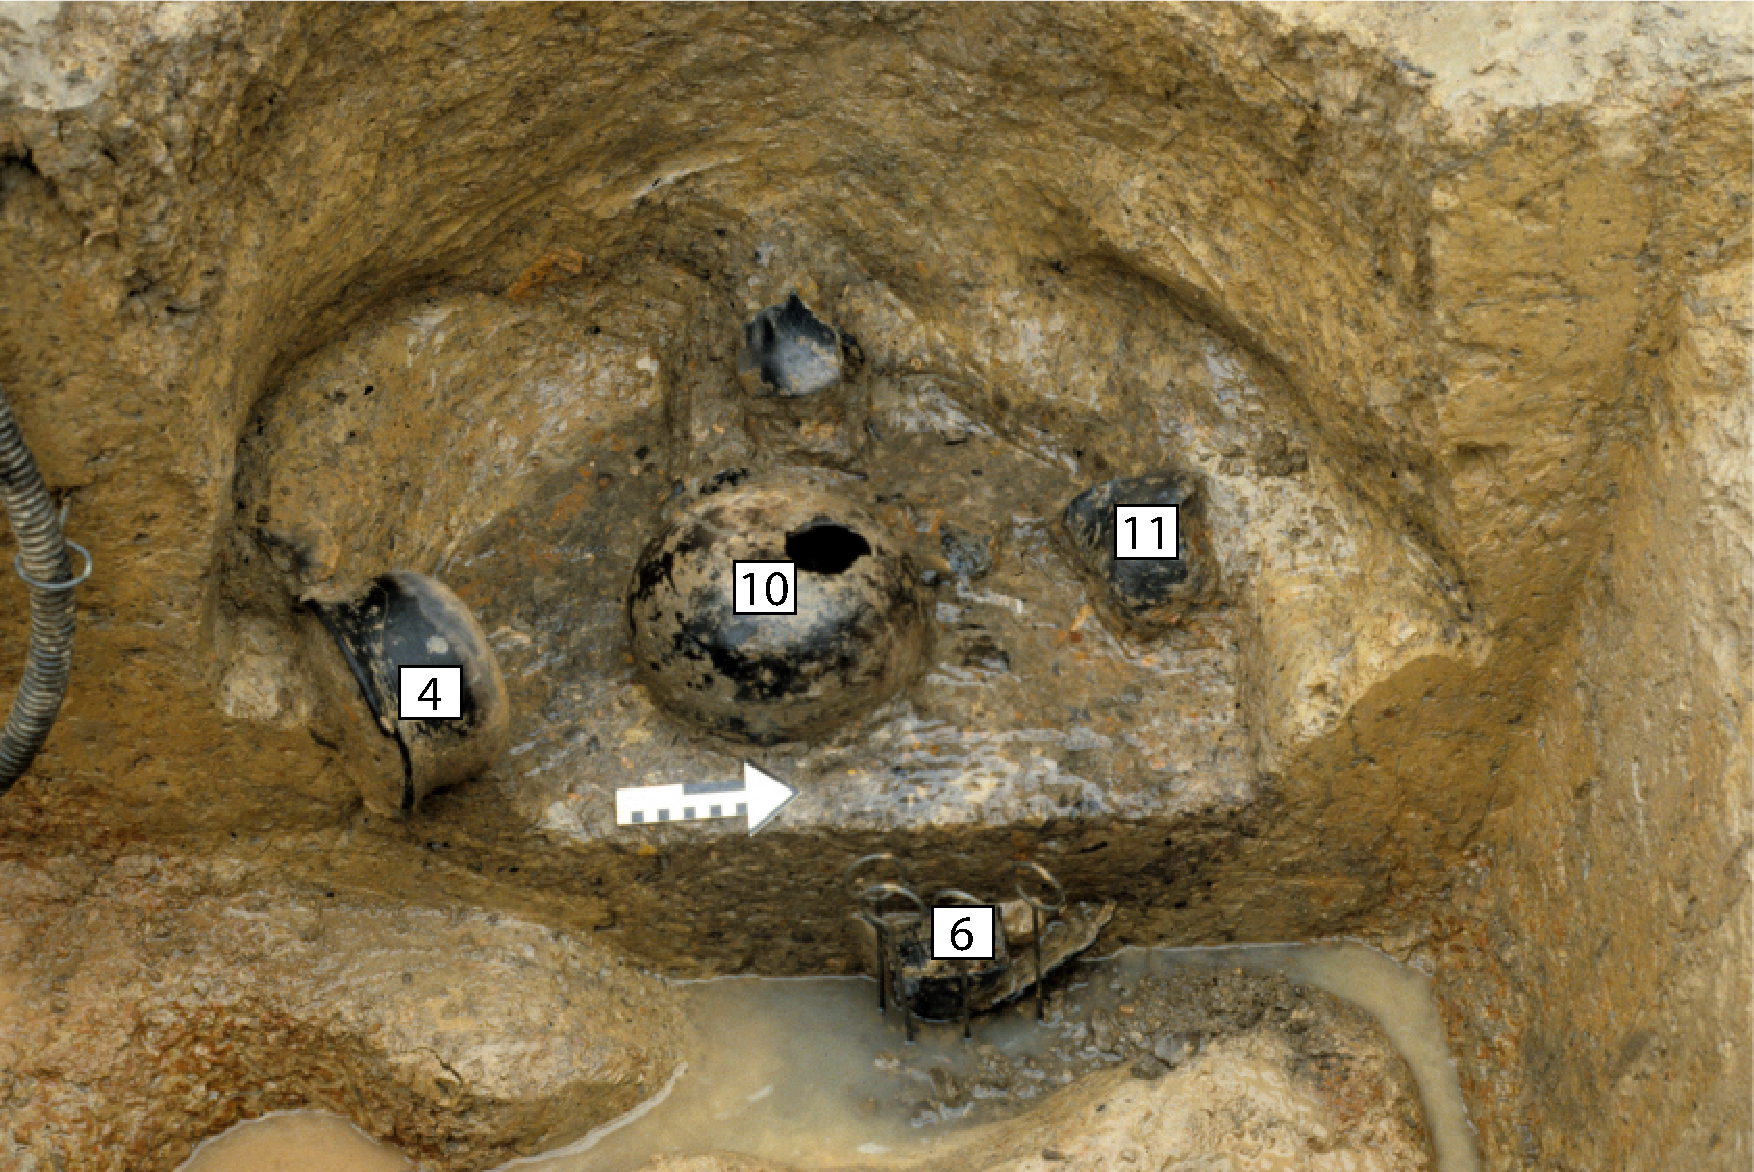
\includegraphics[width = \textwidth]{fig/MUN87-213_T106_H87-06-15.pdf}
		\caption{T106 (Foto: H. Holsten, 1987)}
		\label{fig:MUN87-213_T106_H87-06-15}
	\end{subfigure}
	\begin{subfigure}[t]{\columnwidth}
		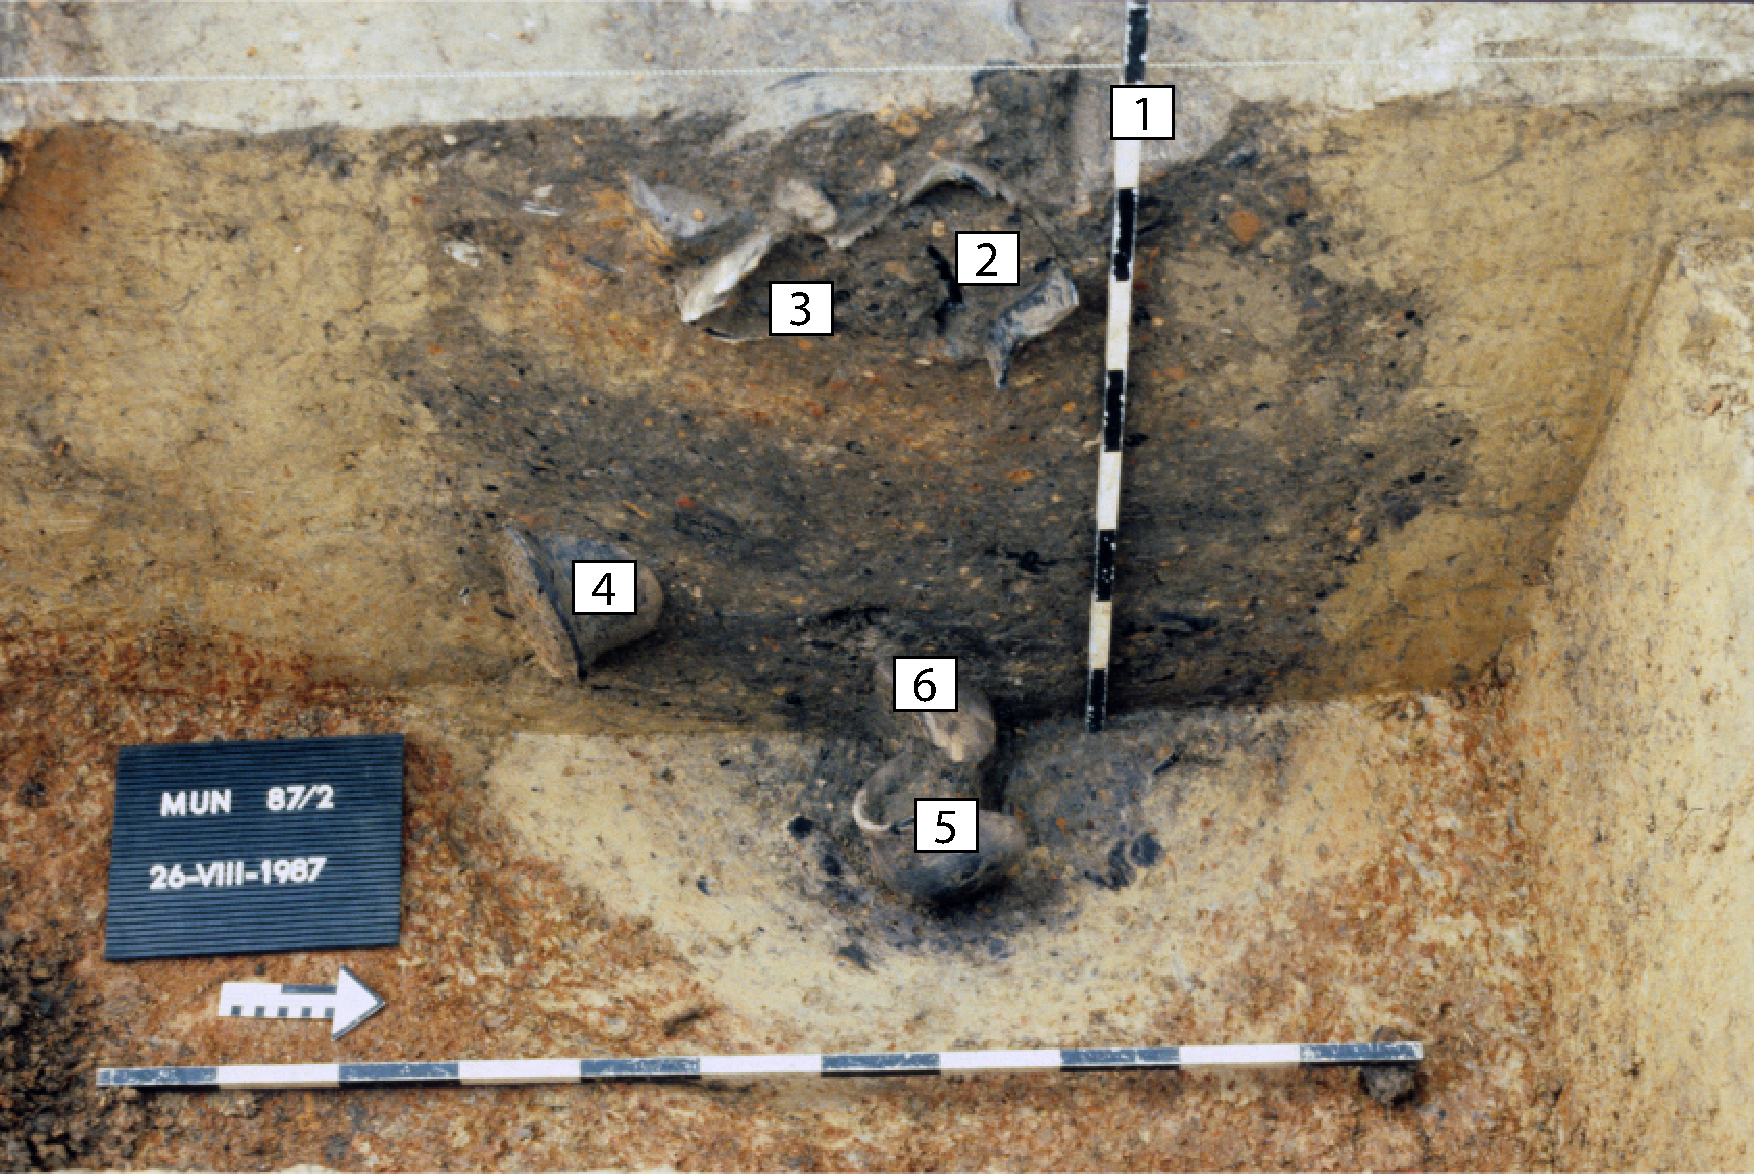
\includegraphics[width = \textwidth]{fig/MUN87-213_T114_H87-06-6.pdf}
		\caption{T114 (Foto: H. Holsten, 1987)}
		\label{fig:MUN87-213_T114_H87-06-6}
	\end{subfigure}\hfill
	\begin{subfigure}[t]{\columnwidth}
		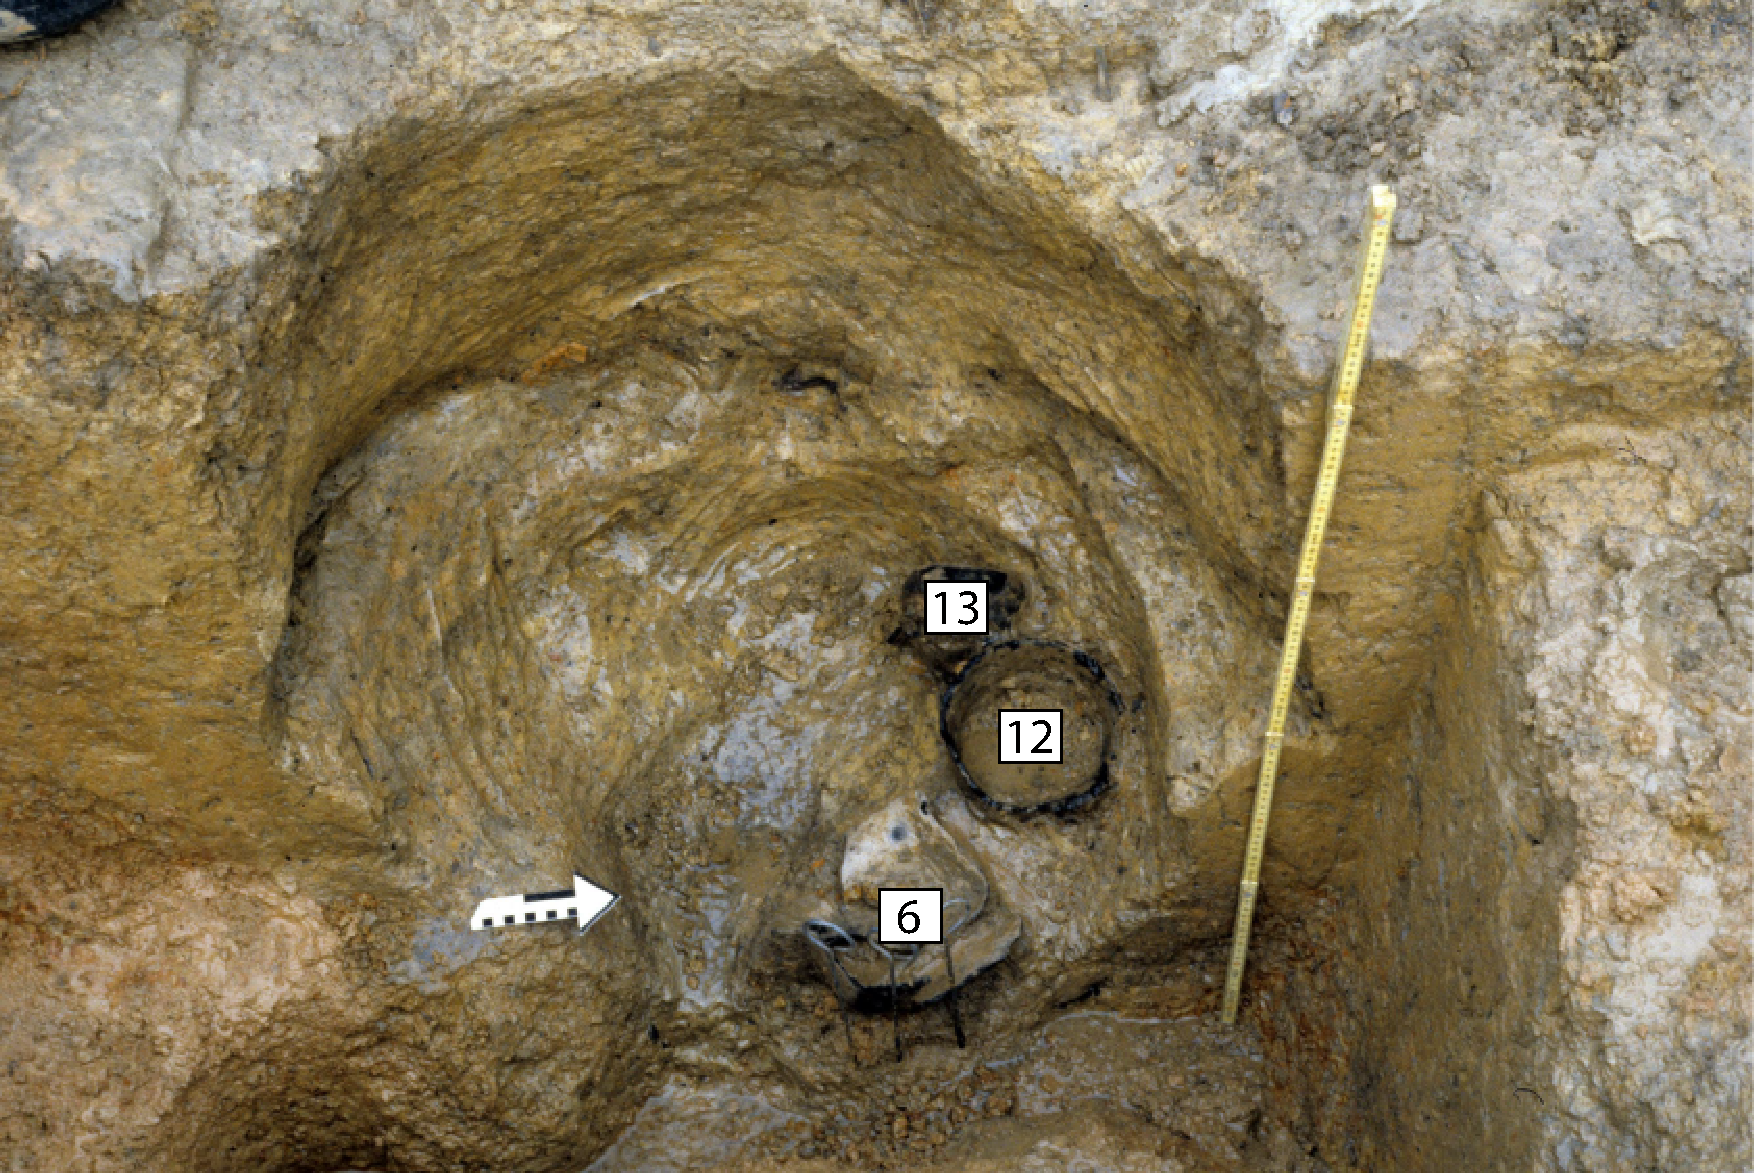
\includegraphics[width = \textwidth]{fig/MUN87-213_T130_H87-06-20.pdf}
		\caption{T130 (Foto: H. Holsten, 1987)}
		\label{fig:MUN87-213_T130_H87-06-20}
	\end{subfigure}	\caption{MUN~87/2-1-3: Abträge der 1. (links) und 2. Hälfte (rechts).}
	\label{fig:MUN87.2-1-3_Plana_Fotos}
\end{figure*}

\begin{figure*}[p]
	\centering
	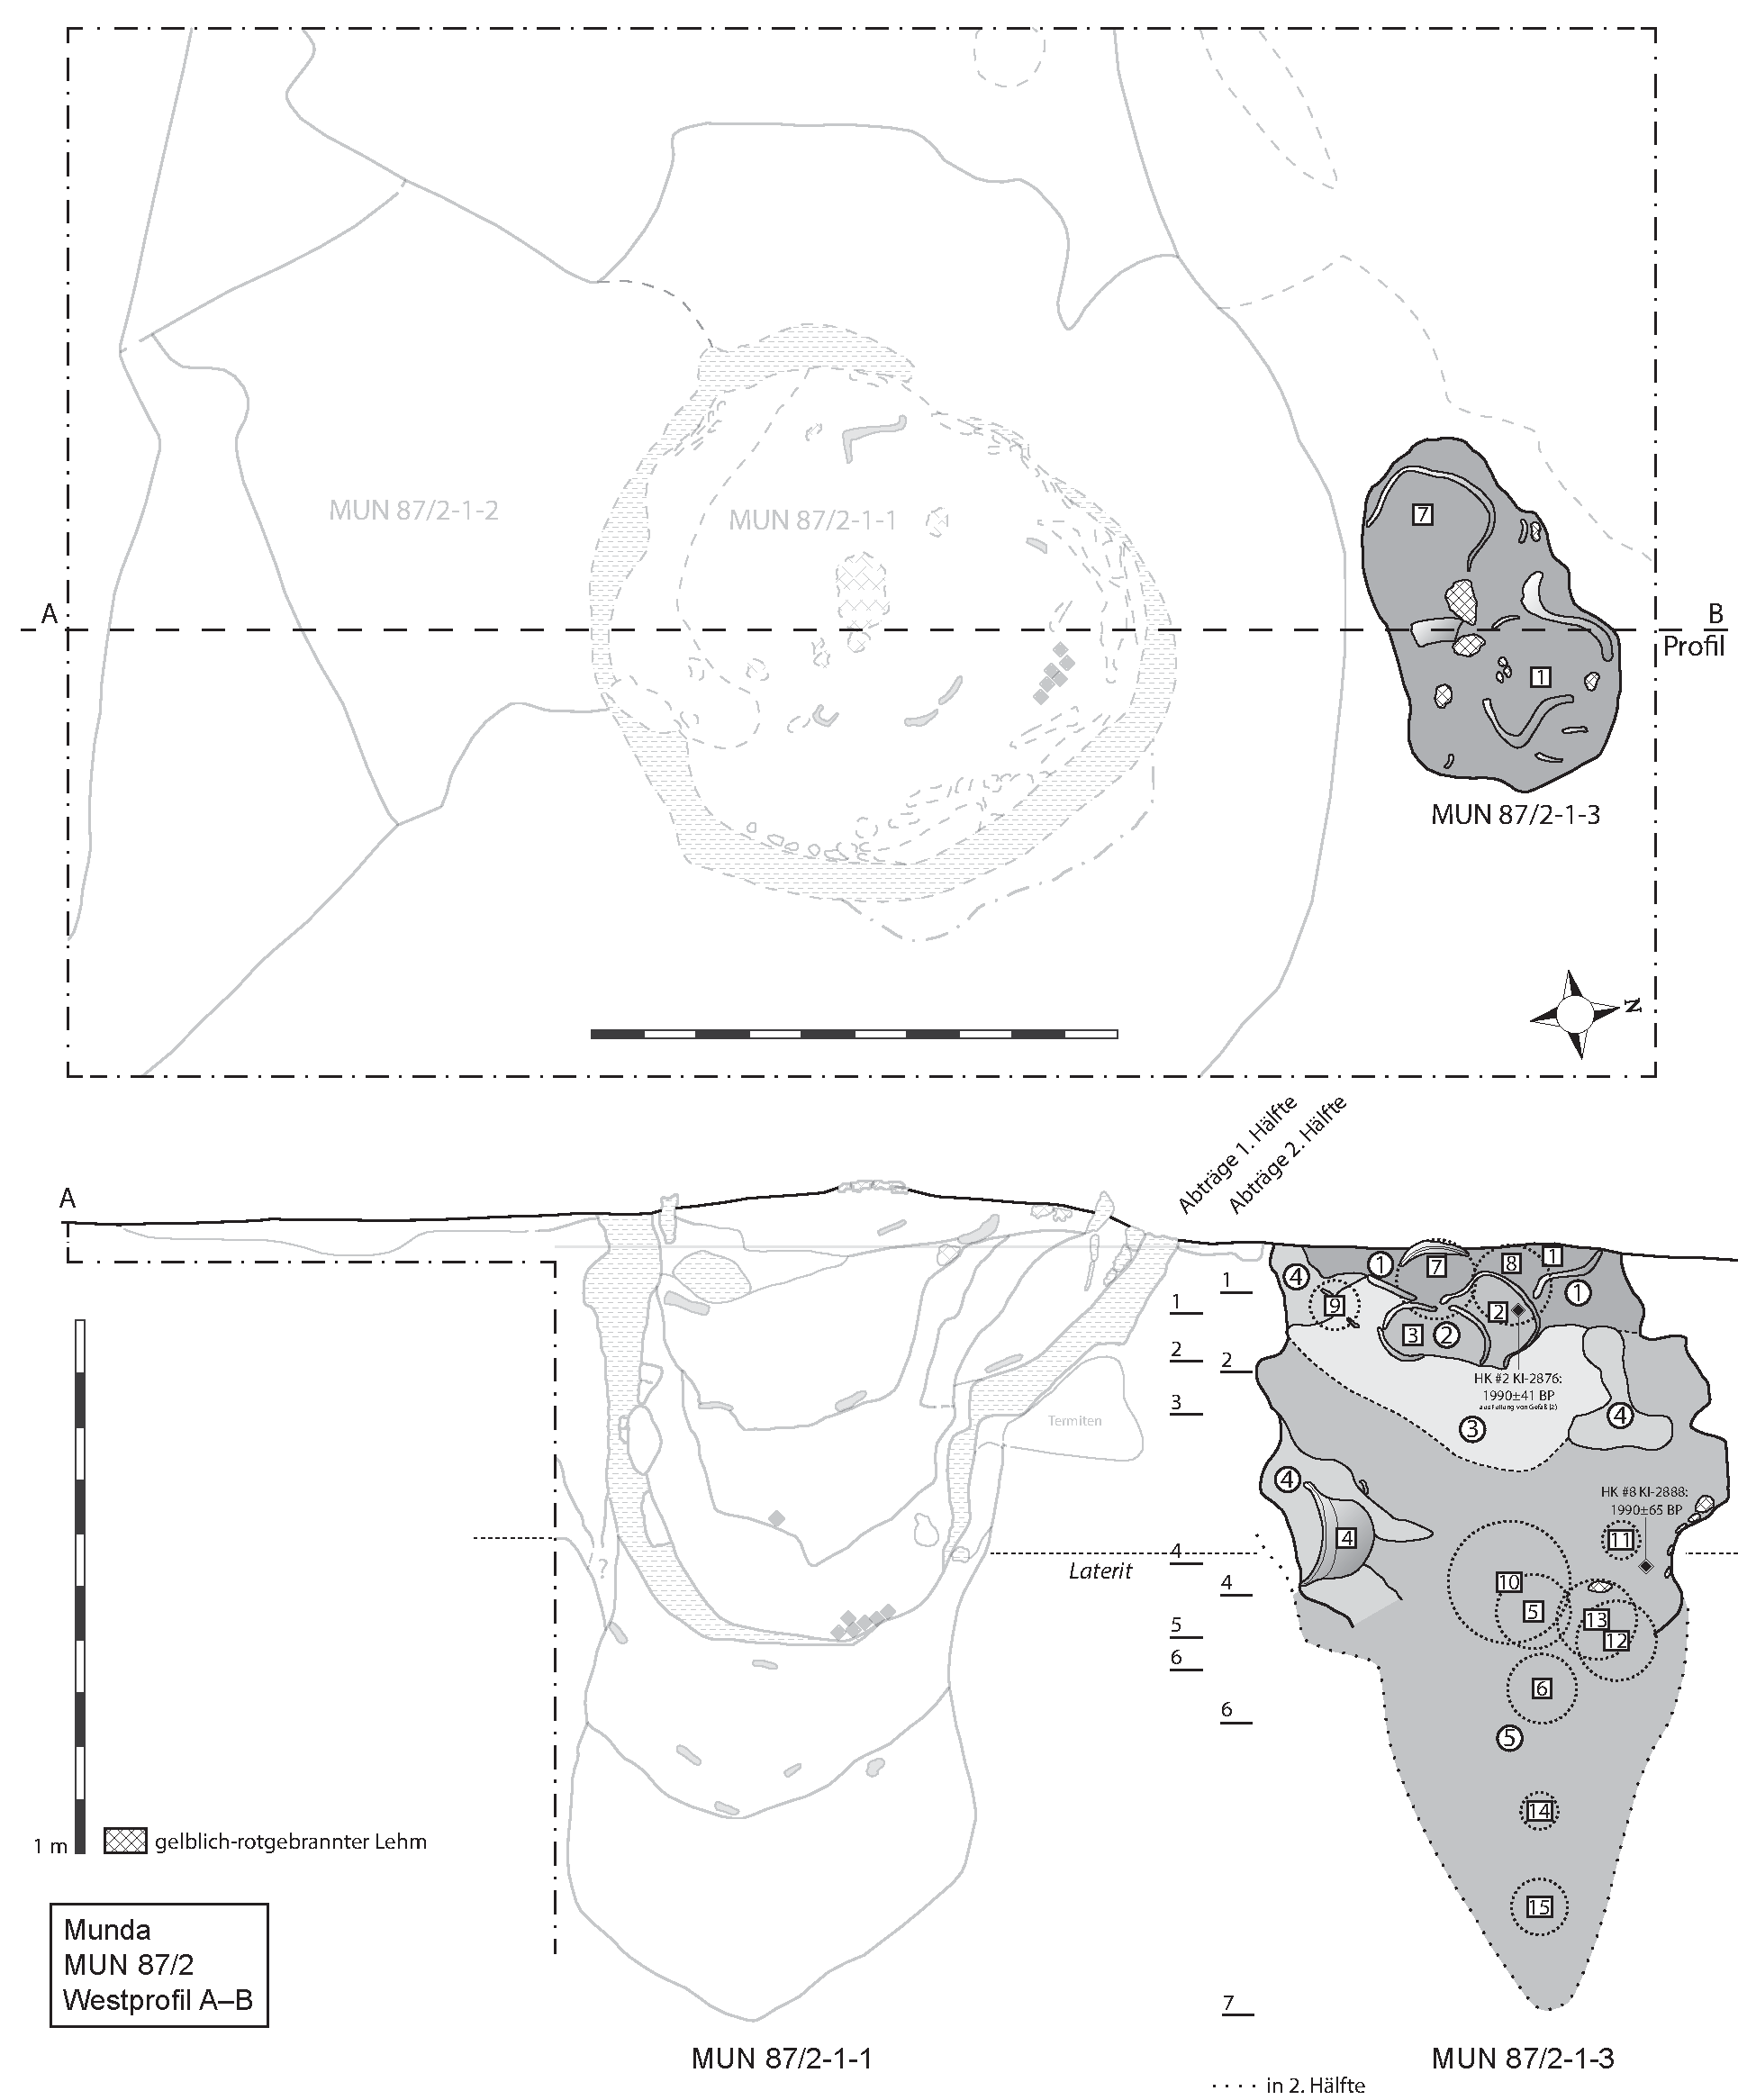
\includegraphics[width=\textwidth]{fig/MUN87-213.pdf}
	\caption{MUN~87/2-1-3: Planum und Profil.}
	\label{fig:MUN87.2-1-3_Planum+Profil_Zeichnung}
\end{figure*}

Die obere Gefäßsetzung besteht aus fünf Schalen des Typs E3 (Taf.~92.1--4, 6), die sich um Gefäß 8 (Taf.~92.8), ein hohes Gefäß mit langer Schulter und ausbiegendem Rand vom Typ B1, und einen Teller oder Deckel mit umbiegendem Rand und \textit{Mittelrippe} (Taf.~93.8) gruppieren (Abb.~\ref{fig:MUN87-213_T41_F87-02-14}--E, \ref{fig:MUN87.2-1-3_Planum+Profil_Zeichnung}).\footnote{Das oberste Verfüllpaket 1 (Abb.~\ref{fig:MUN87.2-1-3_Planum+Profil_Zeichnung}) ist mit rot verziegelten, etwa 1--5\,cm großen Tonbrocken, kleinen Holzkohle-Flittern und vielen, zum Teil komplett erhaltenen verkohlten Ölpalmen-Kernen durchmischt. Zwischen den Gefäßen 2 und 3 fand sich eine Konzentration verkohlter Palmkerne, die so dicht war, dass dazwischen fast kein anorganisches Material vorhanden gewesen sei. Unterhalb der obersten Gefäßsetzung befand sich die etwa 8--10\,cm mächtige Schicht~3, die vorwiegend aus 0,5--1\,cm kleinen roten Lateritpartikeln und etwa 2\,cm großen rot-weiß-verziegelten Tonstücken bestand. Diese zog sich vom südlichen Rand der Eingrabung bis etwa unter die nördliche Kante von Gefäß 2. In der Nähe von Gefäß 9, etwa 0,1\,m unter der Oberfläche, fanden sich mehrere große weiß- bis rotverziegelte Tonbrocken, die stark an die Wandung der Lehmwanne B des benachbarten Befundes MUN~87/2-1-1 erinnern (Kat.-Nr.~16).} Ab etwa 0,5--0,9\,m unter der rezenten Oberfläche formen die Gefäße 4--6 und 10--13 eine zweite Konzentration (Abb.~\ref{fig:MUN87-213_T106_H87-06-15}). Diese besteht aus dem auf der Mündung deponierten Gefäß 10\footnote{Gefäß 10 weist in seinem Boden ein etwa 8\,$\times$\,10\,cm großes Loch auf, das an einer Stelle eine alte, verrundete Bruchkante aufweist. Diese kann dahingehend gedeutet werden, dass das Loch im Zuge einer potenziellen Modifikation des Gefäßbodens vor der Deponierung entstanden sein kann \parencite[siehe][]{Wotzka.1993}.} (Taf.~93.3), um das auf der Seiten liegend sechs Pikunda-Munda-Schalen deponiert wurden (Taf.~92.6, 93.1--2, 4--5, 7). Zwischen den Gefäßen fand sich ein Miniaturgefäß (Taf.~92.9). Dieses weist durchaus stilistische Parallelen zu den Pikunda-Munda-Schalen auf.\footnote{Die kleine Schale ist nur etwa 4\,cm hoch (Taf.~92.9). Sie ist zwar eher \textit{grob} gefertigt, zeigt aber alle Charakteristika einer Pikunda-Munda-Schale: einen ausbiegenden Rand und konkave Wandung sowie runden Bauchumbruch und Boden. Die Verzierung besteht aus horizontalen und vertikalen Ritzlinien und erinnert grob an die häufig im Zusammenhang mit den Schalen des Pikunda-Munda-Stils zu beobachten Schachbrett- oder Leiterornamentik (Tab.~\ref{tab:Verzierungselemente}: 01.1--3).}

Aufgrund der starken Beeinträchtigungen durch das nachlaufende Regenwasser konnten ab dieser Tiefe keine Schichtgrenzen mehr erfasst werden.\footnote{Im Bereich der zweiten Gefäßsetzung enthielt die Verfüllung etwa 1--2\,cm große, rotgebrannte Tonpartikel, etwa 5\,mm große Lateritpartikel, 2--3\,cm große, schwarzgebrannte Ton- oder Lehmstücke und -- im östlichen Randbereich -- etwa 3\,cm große ungebrannte, dunkle Tonstücke. Holzkohle wurde über die gesamte Fläche gleichmäßig verteilt beobachtet. Unmittelbar unterhalb der Gefäßdeponierung war der Bereich nur wenig mit weiß- oder rotverziegelten Tonstücken, kleinsten Lateritflittern und Holzkohlestücken durchsetzt und zudem stark verfestigt. Um die Zone der dunklen Grubenfüllung lag ein etwa 0,1\,m breiter Bereich aus relativ homogenem, sterilem, gelbem, stark tonigen Material, das nach oben keine erkennbare Abgrenzung zum anstehenden gelben Lehm hat (Abb.~\ref{fig:MUN87-213_T114_H87-06-6}).} Bis etwa 0,8\,m unter der rezenten Oberfläche hatte die Grube einen mehr oder weniger zylindrischen Querschnitt, mit annähernd gerader Wandung. Weiter unterhalb lief sie zur Sohle hin spitz zu. An der Sohle fand sich ein einzelnes Gefäß (Taf.~93.6). 

\begin{table*}[tb!]
	\centering{\footnotesize
		\begin{sftabular}{@{}lrrrr@{}}
\toprule
   \textbf{Fundkategorie} &  \textbf{Anzahl} &    \textbf{\%} &  \textbf{Gewicht (kg)} &    \textbf{\%} \\
\midrule
 gebrannter Lehm &      66 &  33,5 &          2,02 &  15,7 \\
         Keramik &     130 &  66,0 &         10,84 &  84,1 \\
          Sonder &       1 &   0,5 &          0,02 &   0,2 \\
\bottomrule
\end{sftabular}
}
	\caption{MUN~87/1-2-3: Anteil verschiedener Fundmaterialien.}
	\label{tab:MUN87-2-1-3_Funde}
\end{table*}

\begin{figure*}[tb!]
	\centering
	\includegraphics[width=\textwidth]{fig/9-14_MUN87-213_Fragmentierung_2.pdf}
	\caption{MUN~87/2-1-1: Fragmentierungsgrad der Scherben (n~=~130; Größenklassen siehe Anm.~\ref{ftn:Keramik_Fragmentierung}).}
	\label{fig:MUN87-213_Fragmentierung}
\end{figure*}

\begin{figure*}[tb!]
	\begin{minipage}{\textwidth}
		\centering{\footnotesize
		\begin{sftabular}{@{}p{.1\textwidth}p{.1\textwidth}p{.3\textwidth}p{.25\textwidth}p{.15\textwidth}@{}}
			\toprule
			\textbf{Lab-Nr} & \textbf{Datum (bp)} & \textbf{Datum (2-Sigma)} & \textbf{Abtrag} & \textbf{Tiefe (unter NP)} \\ 
			\midrule
			KI-2876 & 1990\( \pm \)41 & \parbox[t]{.25\textwidth}{95 v.~Chr.--87 n.~Chr. (94,0\,\%)\\105--120 n.~Chr. (1,4\,\%)} & 2 (HK 2; Palmkern aus Füllung Gef. 2) & 0,5\,m \\ 
			KI-2888 & 1990\( \pm \)65 & 181 v.~Chr.--135 n.~Chr. & Westteil (HK 8) & 1,00\,m \\ 
			\bottomrule 
		\end{sftabular}}
		\captionof{table}{MUN~87/2-1-3: \textsuperscript{14}C-Datierungen.}
		\label{tab:MUN87-213_14C-Daten}
	\end{minipage}
	
	\vspace{1em}
	
	\begin{minipage}{\textwidth}
		\centering
		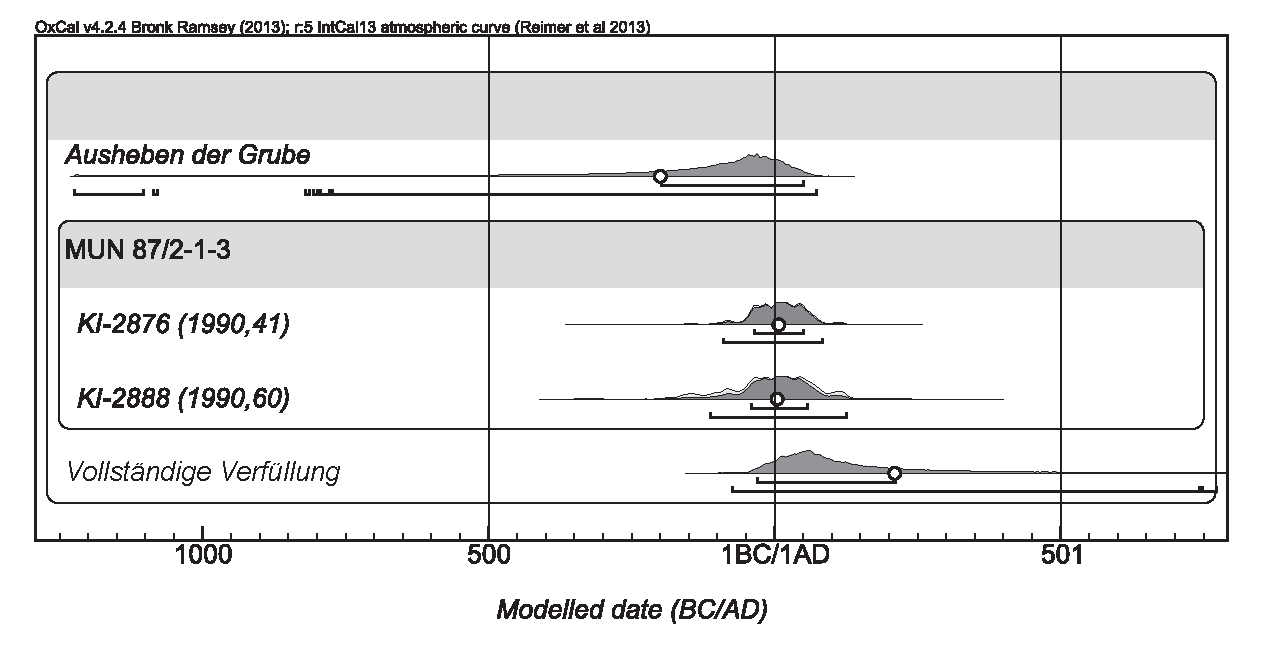
\includegraphics[width = .75\textwidth]{fig/MUN87_2_1_3_14C.pdf}
		\captionof{figure}{MUN~87/2-1-3: Modellierte Datierung der Phasen des Befundes auf Basis der \textsuperscript{14}C-Datierungen.}
		\label{fig:MUN87-2-1-3_14C_OxCal}
	\end{minipage}
\end{figure*}

%\vspace{1.5em}
\noindent Die Grabung erbrachte den folgenden stratigrafischen Befund (Abb.~\ref{fig:MUN87.2-1-3_Planum+Profil_Zeichnung}):
\begin{itemize}[leftmargin=*, labelindent=1.25em, noitemsep, topsep=0pt]
	\item [(1)] 10YR 3/3; schwarz-grau humoses Material mit Holzkohle und verziegelten Tonbrocken
	\item [(2)] 10YR 4/3; Füllmaterial der Keramiksetzung Gef. 1 – Gef. 3, relativ homogenes dunkelbraunes bis dunkelgraues Material mit verziegelten Tonbrocken und verkohlten Palmkernen
	\item [(3)] 10YR 4/3 bis 7,5YR 5/6; rötlich-gelb-graues Material mit vielen kleinen Lateritbrocken, Holzkohle mit ungebrannten gelben Tonstücken, wenig rot-verziegelte Tonbrocken
	\item [(4)] 10YR 5/4; gelblich-graues, tonlinsenartiges Material mit Holzkohle und einigen kleinen rot-verziegelten Tonbrocken
	\item [(5)] 10YR 4/2; relativ homogen durchmischtes dunkelgraues Material mit sehr wenig Keramikfragmenten, dafür aber annähernd vollständigen Gefäßen [Gef. 4 – Gef. 6], Holzkohle und verkohlte Palmkerne, rotverziegelte und teilweise gelbe oder schwarz-braune ungebrannte Tonbrocken enthaltend
\end{itemize}

\columnbreak
\paragraph{Keramik\vspace{.5em}}\mbox{}\\
\begin{tabular}{@{}lrl@{}}
Ausgezählt: & 913\,g & \\ 
Bearbeitet: & 9863\,g & (92\,\%) \\ 
Insgesamt: & 10776\,g & \\ 
\end{tabular}

\vspace{1em}
\noindent Das Fundmaterial besteht, mit Ausnahme von etwa 2\,kg über den gesamten Befund verteilten gebrannten Lehm, ausschließlich aus Keramikgefäßen und zerscherbter Keramik (Tab.~\ref{tab:MUN87-2-1-3_Funde}). Das Gros des Keramik"-inventars setzt sich aus Gefäßen oder großen Gefäßfragmenten zusammen (Abb.~\ref{fig:MUN87-213_Fragmentierung}). Nicht näher ansprechbare oder nicht diagnostische Einzelscherben kommen nur selten vor. Insgesamt 22~GE konnten unterschieden werden, darunter insgesamt acht vollständige Gefäße. Alle GE entsprechen sich formale wie technisch.\footnote{Das Inventar der Grube MUN~87/2-1-3, zusammen mit jenem der benachbarten Grube MUN~87/2-1-1 (Kat.-Nr.~16), dem Verhüttungsbefund MUN~87/3 (Kat.-Nr.~18) und den aus der in der Grabung PIK~87/1 in Pikunda am \mbox{Sangha} erfassten Grube B (Kat.-Nr.~8) stammenden GE bildet die Grundlage für die Beschreibung des Pikunda-Munda-Stils (Kap.~\ref{sec:PKM-Gr}). In keinem anderen Befund konnte eine ähnlich starke stilistische Einheitlichkeit der Gefäßkeramik beobachtet werden.}

Das Inventar wird von 15 kompletten oder in Fragmenten erhalten Schalen des Typs E3 bestimmt. Diese Form ist die diagnostische Form für den Pikunda-Munda-Stil (Kap.~\ref{sec:PKM-Gr}). Die übrigen Gefäßformen sind jeweils nur als Einzelfunde belegt. In der unteren Gefäßkonzentration fand sich ein großes Gefäß mit geschweifter Wandung und ausbiegendem Rand vom Typ E1 (Taf.~93.3). Die obere Gefäßkonzentration enthielt neben den Schalen ein hohes, bauchiges Gefäß mit langer Schulter und kurzem, ausbiegendem Rand vom Typ B1 (Taf.~92.8) sowie eine rundbodige Schale mit gerader Wandung vom Typ I3 (Taf.~92.5). Des Weiteren fand sich hier auch ein Fragment eines Deckels oder Tellers, für den es bislang noch kein Vergleichsstück gibt (Taf.~93.8).\footnote{Es handelt sich um eine Tonplatte mit einem Durchmesser von etwa 30\,cm, die einen umbiegenden, gerade verlaufenden Rand von etwa 3\,cm Höhe aufweist. Zudem führt eine Rippe beziehungsweise Leiste auf das Zentrum der Platte zu. Über die Funktion dieses Stücks können beim aktuellen Quellenstand nur Mutmaßungen angestellt werden.}

Die Randabschlüsse sind zu einem Drittel rund ausgearbeitet und zu einem weiteren Drittel schräg nach außen abgestrichen. Das restliche Drittel umfasst aufgrund schlechter Erhaltung nicht eindeutig ansprechbare Varianten. Gerillte Randabschlüsse, wie sie im Inventar der oberen Verfüllung C im Befund MUN~87/2-1-1 (Kat.-Nr.~16) regelhaft beobachtet wurden (Taf.~91.1--5), finden sich im Material aus MUN~87/2-1-3 nicht. Die meisten Ränder sind konkav ausbiegende und lassen sich dem Typ B2 zuordnen. Alle Gefäße sind grundsätzlich rundbodig, wobei die Grenze zu flachbodigen oder leicht einziehenden Böden häufig fließend sind (siehe Taf.~92.1, 92.5, 93.2--3, 93.5--6).

Die Verzierungen umfassen vor allem horizontale Rillen (Tab.~\ref{tab:Verzierungselemente}: 02.1) und flächiges Schachbrett- beziehungsweise Leitermuster (01.1--2). Regelhaft sind ausschließlich die Ränder und Wandungen verziert. Wie im stratigrafisch älteren Inventar A des benachbarten Komplexes MUN~87/2-1-1 (Kat.-Nr.~16) sind Gefäßunterteile und Standflächen der GE aus MUN~87/2-1-3 regelhaft unverziert.

\paragraph{Datierung}\hspace{-.5em}|\hspace{.5em}%
Aus der Grube MUN~87/2-1-3 liegen zwei Radiokohlenstoffdatierungen vor, die beide in das 2.~Jh. v.~Chr.--2.~Jh. n.~Chr. datieren (Tab. \ref{tab:MUN87-213_14C-Daten}, Abb.~\ref{fig:MUN87-2-1-3_14C_OxCal}). Dieser Zeitraum stimmt nahezu exakt mit dem Alter des unmittelbar benachbarten Befunds MUN~87/2-1-1 und insbesondere der unteren Keramikdeponierung A überein (Kat.-Nr.~16).


\paragraph{Botanisches Material}\hspace{-.5em}|\hspace{.5em}%
Eine Untersuchung der 1987 im Befund entnommenen botanischen Proben, bestehend aus dem Sediment aus den Gefäßen 2, 4, 5, 8, 13 und 15, erfolge 2012--13. In der geschlämmten Gefäßfüllung von Gefäß 2 fand sich ein nahezu vollständig erhaltener Kern einer Raphia-Palme (\textit{Raphia sp.}) \parencite[506, 508 Abb. 7]{Kahlheber.2014}. 


\paragraph{Interpretation}\hspace{-.5em}|\hspace{.5em}%
Die Grabung MUN~87/2-1-3 erfasste eine Deponierung aus acht vollständigen Gefäßen und 14 teilweise sehr großen Gefäßfragmenten des Pikunda-Munda-Stils (Kap.-Nr.~\ref{sec:PKM-Gr}) in einer 1,4\,m tiefen Grube. Das Inventar ist stilistisch gesehen sehr homogen und die Niederlegung in der Grube erfolgte in zwei voneinander getrennten Gruppen: eine in etwa mittig in der Grube sowie eine zweite, direkt unter der rezenten Oberfläche. An der Sohle fand sich noch ein isoliert niedergelegtes Gefäß. Die beiden Gefäßkonzentrationen werden vor allem aus den für den Pikunda-Munda-Stil charakteristischen Schalen des Typs E3 gebildet. Jedoch findet sich im Zentrum der unteren Gefäßkonzentrationen ein großes, bauchiges Gefäß mit ausbiegendem Rand, das auf seiner Mündung stehend deponiert wurde. Der Befund kann durch zwei sich überlappende Radiokohlenstoffdatierungen sicher in das 2.~Jh. v.~Chr.--2.~Jh. n.~Chr. datiert werden. Die Art, in der die vollständigen Gefäße in der Grube lagen, deutet darauf hin, dass es sich um eine Keramikdeponierung handelt, wie sie \textcites{Wotzka.1993}{Wotzka.1995} aus dem Inneren Kongobecken beschreibt.